%!TEX root = ../thesis.tex

\chapter{Multi-dectector wavelength calibration} % Main appendix title
\label{appendix:wavelength_fitting}

In this Appendix we provide an example of multi-detector wavelength calibration.
To try and improve the wavelength calibration on detectors in which limited number of telluric lines fall.


The combined fit is made assigning each detector the position between 0--4095.
In coordinates of the actual {CRIRES} detectors.
A transformation is made into pixel coordinates from the left edge of the first detector by adding the detector gaps (in pixels) to each detector.
The parameters \(gap_{1}\), \(gap_{2}\), \(gap_{3}\) are the 3 gaps between neighbouring detectors gaps and are defined in pixel space as follows:
\[
gap =\begin{cases}
0,                       & ~~~~0=<pxl<1024\\
gap_1,                    & 1024=<pxl<2048\\
gap_1 + gap_2,             & 2048=<pxl<3072\\
gap_1 + gap_2 + gap_3,      & 3072=<pxl<4096
\end{cases}
\]

The pixel widths of these gaps can be fixed to known values (e.g.\ 282, 278, and 275 pixels~\citep{brogi_rotation_2016}) or variable and included in the fitting process.
This is explored below.

\missingfigure{Corner plot of single detector?}

\missingfigure{Corner plot fixed gaps}

\missingfigure{Corner plot variable gaps}

\begin{figure}
    \centering
    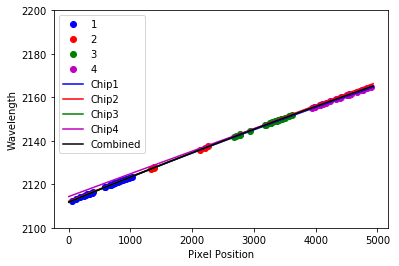
\includegraphics[width=0.45\linewidth]{./figures/appendix/multi_detector_fit}
    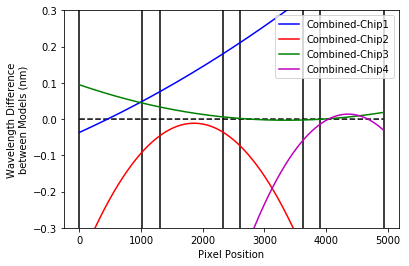
\includegraphics[width=0.45\linewidth]{./figures/appendix/multidector_fit_diff}
    \caption[Multi-detector fit and difference to individual fits.]{Left: Fit of each individual detector and combined quadratic fit.
Right: Difference of each individual fit from the combined detector fit.}
    \label{fig:multidectorfitdiff}
\end{figure}


\begin{figure}
    \centering
    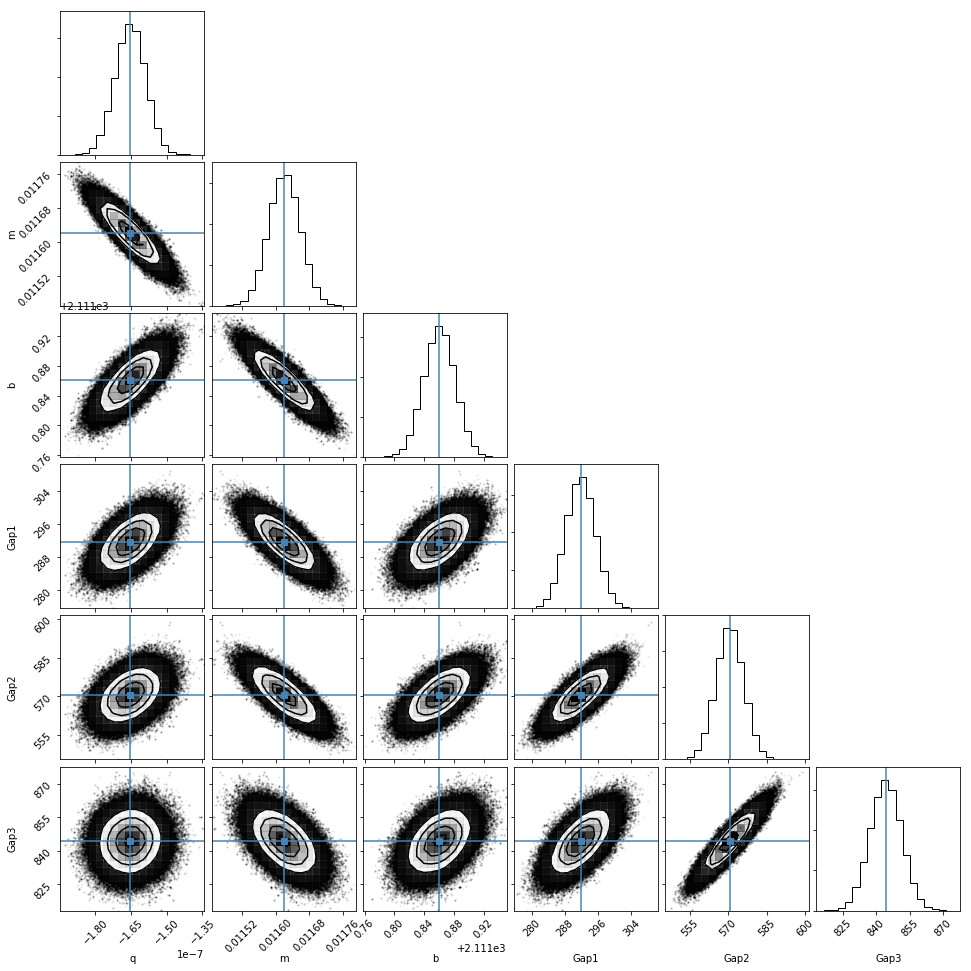
\includegraphics[width=0.5\linewidth]{./figures/appendix/multidetecot_param_fit}
    \caption[Multi-detector parameter correlations.]{Corner plot of emcee combined fitting.
The elliptical point clouds indicate correlation between parameters.}
    \label{fig:multidetecotparamfit}
\end{figure}

This example does not take the \nth{2} position of the spectrum along the detector ot any detector miss-alignments

\cref{tab:example_calibration_parametres} shows the parameters obtains as well as fit statistics for quadratic and cubic fitting.
\textbf{BIC shows that}

\todo{remove vertical lines}
\todo{fill in table}
\begin{table}
    \small
    \caption[Example multi-detector fitting parameters.]{Example multi-detector fitting parameters obtained for HD\,30501 observation 2 under different scenarios.}
    \begin{tabular}{|l|c|c|c|c|c|c|c|c|c|c|c|c|}
    	\toprule
    	  &    \multicolumn{8}{c|}{Individual Detectors}    &    \multicolumn{4}{c|}{Combined}    \\
    	  & \multicolumn{2}{c|}{\#1} & \multicolumn{2}{c|}{\#2} & \multicolumn{2}{c|}{\#3} & \multicolumn{2}{c|}{\#4} & \multicolumn{2}{c|}{Fixed Gaps} & \multicolumn{2}{c|}{Variable Gaps} \\ \midrule
    	a3 (u)    &  -   &    1e-4    &  -   &    &  -   &    &  -   &    &  -   &    &  -   &    blah    \\
    	a2 (q)    &      &    &    &    &    &    &    &    &    &    &    &    blah    \\
    	a1 (m)   &      &    &    &    &    &    &    &    &    &    &    &    blah    \\
    	a0 (b)    & 2111 &    2111    & 2111 &    2111    & 2111 &    2111    & 2111 &    2111    & 2111 &    2111    & 2111 & blah \\
        \(gap_{1}\) &      &    &    &    &    &    &    &    &   1367  & 1367   &   & x\\
        \(gap_{2}\) &      &    &    &    &    &    &    &    &  2700   &  2700  &   & x\\
        \(gap_{3}\) &      &    &    &    &    &    &    &    &   3900 &   3900 &    & x\\
    	\textchisquared{} &    &    &    &    &    &    &    &    &    &    &    &    blah    \\
    	BIC        & -234      &    -234    & -234 &    -234    & -234 &    -234    &    &    -234    & -234 &    -234    & -234 &    blah  \\
        \bottomrule
    \end{tabular}\label{tab:example_calibration_parametres}
\end{table}


\missingfigure{Residuals between individual fitting and the variable gap fits}
